\documentclass{beamer}


\usepackage[english]{babel}
\usepackage[utf8]{inputenc}
\usepackage{thmtools}
\usepackage{stmaryrd}
\usepackage{geometry}
\usepackage{listings}
\usepackage{amsmath,amssymb,amsfonts,amsthm}
\usepackage{graphicx}

%\setbeamertemplate{bibliography item}{\insertbiblabel}
\setbeamertemplate{footline}[frame number]

%\newtheorem{definition}{Definition}[section] % defines the definition environment
%\newtheorem{theorem}{Theorem}[section] % defines the theorem environment
%\newtheorem{lemma}{Lemma}[section]
%\newtheorem{proof}{Proof}[section] % defines the proof environment

% Sets and set operation
\newcommand{\R}{\mathbb{R}} % the reals
\newcommand{\Z}{\mathbb{Z}} % the integers
\newcommand{\N}{\mathbb{N}} % the natural numbers
\renewcommand{\S}{\mathbb{S}} % state space
\newcommand{\leqD}{\sqsubseteq_{D}} % cpo
\newcommand{\leqL}{\sqsubseteq_{L}} % cpo
%\newcommand{\pot}[1]{\mathcal{P}(#1)} % power set

\newcommand{\E}{\mathbb{E}}

% Programs
\newcommand{\smtx}[1]{\left\llbracket #1 \right\rrbracket} % semantic brackets
\newcommand{\res}[2]{\left\langle #1 \right\rangle_{#2}} % restriction
\newcommand{\resP}[1]{\res{#1}{B}} % restriction to B
\newcommand{\resN}[1]{\res{#1}{\lnot B}} % restriction to not B
\newcommand{\nop}{\textit{skip}} % skip statement
\newcommand{\abort}{\textit{diverge}} % abort statement
\newcommand{\ifp}[3]{\textit{if}\,(#1) \, \{ \, #2 \, \} \, \textit{else} \, \{ \, #3 \, \} } % if statement
\newcommand{\while}[2]{\textit{while}\,(#1) \{#2\}} % while loop

\newcommand{\wh}{\operatorname{wh}_{B, P}}
\newcommand{\hh}{\operatorname{H}_{B, P}}
\newcommand{\ww}{\operatorname{ww}_f}
\renewcommand{\wp}[1]{\operatorname{wp}\l( #1 \r)}

% Convenience
\newcommand{\qu}{\frac{1}{4}} % 1 / 4
\newcommand{\half}{\l( \frac{1}{2} \r)} % (1 / 2)
\newcommand{\hf}{\frac{1}{2}} % 1 / 2
\newcommand{\IH}[1]{\overset{IH}{#1}} % for induction hypothesis
\newcommand{\pair}[1]{\left( #1 \right)} % round parentheses
\renewcommand{\l}{\left} % short left
\renewcommand{\r}{\right} % short right
\newcommand{\infsum}{\sum\limits_{i = 0}^{\infty}} % sum from 0 to inf over variable i
\newcommand{\multisum}[1]{\sum\limits_{s \in \N^k} #1 X_1^{s_1} \cdots X_k^{s_k}}
\newcommand{\Xok}{X_1^{s_1} \cdots X_k^{s_k}} % variables X_1 to X_k
\newcommand{\explain}[1]{\hspace*{2em} \l(\text{\small #1}\r)} % explanation in proof, indented line with smaller text
\newcommand{\where}{, \text{ where }}

% Display
\renewcommand{\vert}{\ | \ }


\addtolength{\jot}{0.5em} % increase align line spacing
%\setlist{itemsep=20pt}
\newcommand{\itemspacing}[1]{\setlength\itemsep{#1}}

\newcommand{\HRule}{\rule{\linewidth}{0.5mm}}	% horizontal lines for title

% math symbol for general cartesian product, copied from kpfonts.sty, lines 611 & 1495
\DeclareSymbolFont{largesymbolsA}{U}{jkpexa}{m}{n}
\DeclareMathSymbol{\bigX}{\mathop}{largesymbolsA}{16}
\newcommand{\bigtimes}{\bigX} % redundant declaration to make texstudio recognize \bigtimes


% (re)define square subsets
\DeclareFontFamily{U}{mathb}{\hyphenchar\font45}
\DeclareFontShape{U}{mathb}{m}{n}{
	<5> <6> <7> <8> <9> <10> gen * mathb
	<10.95> mathb10 <12> <14.4> <17.28> <20.74> <24.88> mathb12
}{} 
\DeclareSymbolFont{mathb}{U}{mathb}{m}{n}
\DeclareMathSymbol{\sqsubseteq} {3}{mathb}{"84}
\DeclareMathSymbol{\sqsupseteq} {3}{mathb}{"85}
\DeclareMathSymbol{\sqsubsetneq}{3}{mathb}{"88}
\DeclareMathSymbol{\sqsupsetneq}{3}{mathb}{"89}


\lstset{language=Java} % lstlisting language
%\setlist[description]{font=\normalfont\space} % normal font in description env. labels




\title{Extending Probability Generating Function Semantics to Negative Variable Valuations}
\subtitle{Bachelor Colloquium}
\date{12.04.2016}
\author{Simon Feiden}


\begin{document}
	
	
\maketitle

%\begin{frame}
%	\tableofcontents
%\end{frame}


\section{Motivation}
Probabilistic programs are programs that do not always produce the same result for one set of inputs.
This is achieved by the usage of probabilistic operations, which are embedded into the programming language itself.
%Contrary to randomised programs, probabilistic programs do not rely on an external source of randomness, but use this inherent mechanism to make random decisions.
Applications are in testing, where error rates can be modelled easily using probabilistic programs.
They can also be used to solve problems that are very hard to solve or are not solvable at all using classical programming paradigms \cite{motwani:randomized}. \\
Because of its non-deterministic nature, code written by using a probabilistic programming language is not easily verified just by reading and understanding.
To obtain insights about properties such as correctness and termination probability, a formal method is necessary.
It should allow to derive statements about the aforementioned properties.
Unlike program code, which describes how something is calculated, the formal method must keep track of what happens while a program is executed.
What happens, or the meaning of the process, is called the program's semantics.
One idea to define a semantics is to keep track of all possible variable valuations, called the program states. \\
Probabilistic programs are not deterministic.
Consequently, program states only have a probability of appearing as result of the whole computation.
To capture all program states with their probabilities, \emph{probability generating functions} (PGFs) can be used.
This thesis is built on work of Scherbaum \cite{clara:pgf}, which uses \emph{formal power series} as PGFs.
These PGFs lack the possibility of having variables with negative values.
Thus, even simple programs that use subtraction cannot be represented by one of those PGFs.
In this work, we will extend Scherbaum's model, so that variables can also have negative values.
Later, we will show that the newly derived semantics is equivalent to an already established one which was introduced by McIver and Morgan.~\cite{mciver:abstraction_refinement}.



\section{Preliminaries}
\subsection{Formal Power Series}
A formal power series (FPS) \cite{wilf:generatingfunctionology} is a polynomial of degree $\infty$ over one variable, most commonly $X$.
A formal power series $F$ is an object of the form
\[ F = a_0 X^0 + a_1 \cdot X^1 + a_2 X^2 + \ldots = \infsum a_i X^i \]
The coefficients $a_i$ are real numbers.
When dealing with a formal power series $F$, $F$ is not meant to be a function.
This means that $X$ is not necessarily substituted by a value, so properties like convergence are ignored. \\
Formal power series can be added and multiplied.
Addition comes in a very natural way, it is done componentwise:
\[ F + G = \infsum a_i X^i + \infsum b_i X^i
	= \infsum (a_i + b_i) X^i \]
Multiplication is more complicated.
\[ F \cdot G = \infsum c_i X^i \where c_i = \sum_{k = 0}^{i} a_k b_{i-k} \]
The product of two formal power series is always defined because the sum of every coefficient $c_i$ consists of only finitely many elements.
In fact, the formal power series form a ring under addition and multiplication.
The ring's additive and multiplicative identities are
\[ 0 = \infsum 0 X^i \text{ and } 1 = 1 X^0 + 0 X^1 + 0 X^2 + \ldots \]
Later on, we will need another operation on formal power series, the scalar multiplication:
\[ \alpha \cdot F = \infsum (\alpha \cdot a_i) X^i \where \alpha \in \R \]
Obviously, scalar multiplication always has a formal power series as its result.
Some formal power series even have a closed form.
A closed form is desirable because it eases readability and calculation.
As an example, let us have a look at the geometric series.
It comes up often and is defined as follows:
\[ G = 1 X^0 + p X^1 + p^2 X^2 + \ldots = \infsum p^i X^i \where |p| < 1 \]
The closed form of this series is
\[ G = \frac{1}{1 - pX} \]
This means that $1 - pX$ is the multiplicative inverse of $G$.
In other words: $G \cdot (1 - pX) = 1$ where 1 on the right hand side is the identity of the ring, as given above.
In fact, the equation also holds if $|p| > 1$ because we do not consider convergence of the sums.
$|p| < 1$ must only hold if we want to call a PGF a geometric series.

\subsubsection*{Absolute Value}
Despite ignoring convergence etc.\ during operations on formal power series, it is sometimes useful to know about the sum of all coefficients.
Summing all coefficients is comparable to substituting the formal variable $X$ with 1, or evaluating the series at 1.
It may happen that the sum diverges, but when it does not, it can have a meaningful interpretation as we will see later.
Given a formal power series $G = \infsum a_i X^i$, define the absolute value $|G|$ as the sum of all its coefficients:
\[ |G| = \infsum a_i \]
Here, we have another reason why closed forms of formal power series are interesting.
Consider the geometric series
\[ G = \infsum \half^i X^i \]
Now, calculate the absolute value of both the closed and non closed form.
\begin{align*}
	|G| &= \l| \infsum \half^i X^i \r| = \infsum \half^i = 2 \\
	\\
	|G| &= \l| \frac{1}{1 - \frac{1}{2} X} \r| = \frac{1}{1 - \frac{1}{2}} = 2
\end{align*}
Of course, they both have the same value because they are equivalent.
Nonetheless, calculating the absolute value of the closed form is easier, since fractional arithmetic is simpler than reasoning about the value of a series. \\
Note that, although the notation may suggest it, the absolute value is \emph{not} a norm in the classical sense.
It is rather a linear function because the following holds:
\[ |a \cdot G + F| = a \cdot |G| + |F| \]

\subsection{Multivariate Formal Power Series}
Multivariate formal power series are similar to formal power series except they can have more than one formal variable.
A multivariate formal power series $G$ is an object of the form
\[ G = \multisum{a_s} \where k \in \N_{> 0} \]
Addition is defined componentwise as it is for formal power series.
\[ F + G = \multisum{a_s} + \multisum{b_s} = \multisum{(a_s + b_s)} \]
Multiplication again is more complicated, but is defined in a similar fashion as for formal power series.
\begin{align*}
	& F \cdot G = \multisum{c_s} \\
	& \text{where } c_s = \sum_{\substack{n \in \N^k \land \\
		n_j \leq s_j \text{ for all } j \in \{1,\dots,k\}}}
		a_{n_1, \dots, n_k} \cdot b_{s_1 - n_1, \dots, s_k - n_k}
\end{align*}
The concepts of scalar multiplication and absolute value are defined as expected for multivariate formal power series.

\subsection{Formal Power Series As Probability Generating Functions}
We mentioned earlier that formal power series can be used as probability generating functions.
Given a formal power series
\[ G = \multisum{\mu_s} \]
$\mu_s$ is interpreted as the probability that the random variables $X_1, \ldots, X_k$ have the values $s_1, \ldots, s_k$. In other words
\[ \mathcal{P}(X_1 = s_1, \ldots, X_k = s_k) = \mu_s \]
When used as PGFs, formal power series can still be added, scaled and multiplied.

\subsection{Programs}
In order to reason about probabilistic programs by means of a semantics, we need to define a programming language.
We will use the same language as in \cite{clara:pgf}.
It consists of seven different operations that can be combined to form programs.

\subsubsection*{Basic Operations}
\begin{enumerate}
	\item $\nop$ \vspace{0.3\baselineskip} \\
		The $\nop$ operation does nothing and simply goes on to the next operation.
		It is useful in composite operations.
	\item $\abort$ \vspace{0.3\baselineskip} \\
		The $\abort$ operation does not terminate.
	\item ${X := e}$ \vspace{0.3\baselineskip} \\
		The variable $X$ is assigned the value of $e$.
		$e$ is an expression over the program variables that is evaluated right before the assignment to $X$.
\end{enumerate}
\subsubsection*{Composite Operations}
Here, $P, P_1$ and $P_2$ are programs and $B$ is a Boolean condition.
\begin{enumerate}
	\item ${P_1; P_2}$ \vspace{0.3\baselineskip} \\
		The concatenation $P_1; P_2$ means to first execute $P_1$ and then $P_2$.
	\item $\ifp{B}{P_1}{P_2}$ \vspace{0.3\baselineskip} \\
		If the current variable valuations satisfy the condition $B$ then $P_1$ is executed, otherwise $P_2$ is executed.
	\item $\{P_1\}[p]\{P_2\}$ for some $p \in [0, 1]$ \vspace{0.3\baselineskip} \\
		This statement is called probabilistic choice and is what distinguishes this programming language from classical ones.
		Either $P_1$ or $P_2$ is executed at random.
		$P_1$ is executed with probability $p$ and $P_2$ is executed with probability $1-p$.
	\item $\while{B}{P}$ \vspace{0.3\baselineskip} \\
		The \emph{loop body} $P$ is repeatedly executed until the \emph{loop condition} $B$ is no longer satisfied by the program variables.
\end{enumerate}

\subsection{PGF Semantics}
In \cite{clara:pgf}, a semantics for probabilistic programs with multivariate power series as probability generating functions is introduced.
In the following, let $P$ be a program and $G$ be a PGF with
\[ G = \multisum{\mu_s} \]
where $k$ is equal to the number of program variables used in $P$. \\
Every element of the sum in $G$ corresponds to one possible program state with its probability of occurrence.
For example \[ \frac{1}{3} X_1^2 X_2^5 \] means that with probability $\frac{1}{3}$, variable $X_1$ has value 2 and variable $X_2$ has value 5.
It is easy to see that the absolute value $|G|$ must be less than or equal to 1, because otherwise the total probability of all program states would be greater than 1.
% $|G|$ is also the probability that a program terminates.
Note that the sum of a PGF ranges over $\N^k$, so a variable cannot have a negative value.
Assignments or rather expressions are constrained to only evaluate to positive values. \\
Every $P$ has a corresponding function, denoted by $\smtx{P}$, that transforms an initial PGF into the PGF that results from executing $P$.
These functions are defined next.
\subsubsection*{Basic Operations}
\begin{enumerate}
	\item $\smtx{\nop}(G) = G$
	\item $\smtx{\abort}(G) = 0 = \multisum{0}$
	\item $\smtx{X_j := e}(G) = \sum\limits_{s \in \N^k} \mu_s X_1^{s_1} \cdots X_j^{e(s)} \cdots X_k^{s_k}$
	\item
	$\resP{G} = \sum\limits_{s \in \N^k} \begin{cases}
	\mu_s X_1^{s_1} \cdots X_k^{s_k} &\text{if } s \models B \\
	0 & \text{otherwise}
	\end{cases}$ \\
	\\
	\item[] Above, $s$ is an element of $\N^k$.
	$s_j$ refers to the $j$th components of $s$.
	Of course, $1 \leq j \leq k$.
\end{enumerate}
\subsubsection*{Composite Operations}
Here, $P,\ P_1$, and $P_2$ are programs and $B$ is a Boolean condition.
\begin{enumerate}
	\item $\smtx{P_1; P_2}(G) = \smtx{P_2}( \smtx{P_1}(G) )$
	\item $\smtx{ \{P_1\}[p]\{P_2\} }(G) = p \cdot \smtx{P_1}(G) + (1-p) \cdot \smtx{P_2}(G)$
	\item $\smtx{\ifp{B}{P_1}{P_2}}(G) = \smtx{P_1}(\resP{G}) + \smtx{P_2}(\resN{G})$
	\item $\smtx{\while{B}{P}}(G) = \sup\limits_{n \in \N}
		\l\{ \resN{\operatorname{H}_{P, B}^n(G)} \r\}
		\where \operatorname{H}_{P, B}(G) = \smtx{P}(\resP{G}) + \resN{G}$ \\
		$\operatorname{H}_{P, B}$ represents a single iteration of the loop body.
\end{enumerate}
Similar to how programs are concatenated to form longer programs, their individual semantics functions are composed to form the semantics function of the longer program. \\
If $G'$ results from executing a program $P$ on an initial PGF $G$, i.e. $G' = \smtx{P}(G)$, then $|G'|$ is the termination probability of $P$ given the initial distribution.
A simple example is $\abort$.
Applying $\abort$ to any PGF always results in 0, which has absolute value 0, meaning its termination probability is 0.
This is exactly how $\abort$ is defined.
Later, we will see loops that have a termination probability of less than 1.


\section{Semantics}
\begin{frame}{PGFs and Programs}
	
	\begin{columns}
		\begin{column}{0.5\textwidth}
			\begin{itemize}[<+->]
				\itemspacing{10pt}
				\item $ G = \alert<+(1)>{0.4} \alert<+(-1)>{X^1 Y^0}
					+ \alert<+(1)>{0.6} \alert<+(-1)>{X^4 Y^4} $
				\item $\nop$
				\item<.-> $\abort$
				\item<.-> ${X := e}$
			\end{itemize}
		\end{column}
		\begin{column}{0.5\textwidth}
			\begin{itemize}[<.->]
				\itemspacing{10pt}
				\item<+-> ${P_1; P_2}$
				\item $\ifp{B}{P_1}{P_2}$
				\item $\{P_1\}[p]\{P_2\}$
				\item $\while{B}{P}$
			\end{itemize}
		\end{column}
	\end{columns}
\end{frame}

%\begin{frame}
%\frametitle{PGF Semantics}
%	\begin{itemize}
%		\itemspacing{20pt}
%		\item<1-> $\smtx{\nop}(G) = G$
%		\item<2-> $\smtx{\abort}(G) = 0$
%		\item<3-> $\smtx{X_j := e}(G) = \sum\limits_{s \in \N^k} \mu_s X_1^{s_1}
%			\cdots X_j^{e(s)} \cdots X_k^{s_k}$
%		\item<4->
%			$\resP{G} = \sum\limits_{s \in \N^k} \begin{cases}
%				\mu_s X_1^{s_1} \cdots X_k^{s_k} &\text{if } s \models B \\
%				0 & \text{otherwise}
%			\end{cases}$
%		\item<5-> $ \res{0.4 X^1 Y^0 + 0.6 X^4 Y^4}{X = 1} = 0.4 X^1 Y^0 $
%	\end{itemize}
%\end{frame}
%
%\begin{frame}
%	\frametitle{PGF Semantics}
%	\begin{itemize}
%		\itemspacing{20pt}
%		\item<1-> $\smtx{P_1; P_2}(G) = \smtx{P_2}( \smtx{P_1}(G) )$
%		\item<2-> $\smtx{ \{P_1\}[p]\{P_2\} }(G) = p \cdot \smtx{P_1}(G) + (1-p) \cdot \smtx{P_2}(G)$
%		\item<3-> $\smtx{\ifp{B}{P_1}{P_2}}(G) = \smtx{P_1}(\resP{G}) + \smtx{P_2}(\resN{G})$
%		\item<4-> $\smtx{\while{B}{P}}(G) = \sup\limits_{n \in \N}
%		\l\{ \resN{\operatorname{H}_{P, B}^n(G)} \r\} $
%	\end{itemize}
%\end{frame}


\section{Extended Semantics}
\begin{frame}
	\frametitle{Challenges}
	\begin{itemize}
		\itemspacing{20pt}
		\item<1-> Extension to negative variable valuations
		\item<2-> Use formal power series
		\item<3-> Usage of closed forms (requires a ring)
	\end{itemize}
\end{frame}

\begin{frame}
	\frametitle{Extended PGFs}
	\begin{itemize}[<+->]
		\itemspacing{20pt}
		\item $ \sum\limits_{s \in \alert<+>{\N^k} } \mu_s \Xok $
		\item $ \sum\limits_{s \in \alert<.>{\Z^k} } \mu_s \Xok $
		\item No ring, no closed forms.
		\item Solution: Use PGFs for partitions of the state space.
	\end{itemize}
\end{frame}

\begin{frame}
	\frametitle{Partitions}
	\begin{columns}
		\begin{column}{0.5\textwidth}
			\begin{itemize}
				\itemspacing{10pt}
				\item<1-> One variable X
				\item<2-> State space is $\Z$.
				\item<3-> Partitions are \\
					$\phantom{-}\N$ \\
					$-\N_{> 0}$ \\
					$\phantom{\N}$ \\ % empty lines for alignment with second column
					$\phantom{\N}$
			\end{itemize}
		\end{column}
		\begin{column}{0.5\textwidth}
			\begin{itemize}
				\itemspacing{10pt}
				\item<4-> Two variables X, Y
				\item<5-> State space is $\Z^2$.
				\item<6-> Partitions are \\
					$\phantom{-}\N_{\phantom{> 0}} \times \phantom{-}\N  $  \\
					$          -\N_{> 0}				   \times \phantom{-}\N  $  \\
					$\phantom{-}\N_{\phantom{> 0}} \times           -\N_{> 0}$  \\
					$          -\N_{> 0}				   \times           -\N_{> 0}$
			\end{itemize}
		\end{column}
	\end{columns}
\end{frame}

\begin{frame}
	\frametitle{Partitions}
	\begin{itemize}[<+->]
		\item $ S_1, S_2, \ldots, S_{2^k} $
		\item $ \sum\limits_{s \in \alert<.>{S_1}} \mu_s \Xok, $ \\[10pt]
			\uncover<+->{
					$ \sum\limits_{s \in \alert<.>{S_2}} \mu_s \Xok, $ \\[10pt]
			}
			\uncover<+->{
					$ \vdots $ \\[10pt]
					$ \sum\limits_{s \in \alert<.>{S_{2^k}}} \mu_s \Xok $
			}
	\end{itemize}
\end{frame}

\begin{frame}
	\frametitle{Semantic Tuples}
	\begin{definition}[Semantic Tuple]
		Let $P$ be a program of $k$ variables.
		A \emph{semantic tuple} $T_G$ is an object of the form
		\[ T_G = \l( \sum_{s \in \alert<1>{S_1}} \mu_s \Xok, \ldots,
		\sum_{s \in \alert<1>{S_{2^k}}} \mu_s \Xok \r) \]
	\end{definition}
	\begin{itemize}
		\itemspacing{10pt}
		\item<2-> Number of entries grows exponentially.
		\item<3-> Use extended PGFs: $ \sum\limits_{s \in \Z^k} \mu_s \Xok $
	\end{itemize}
\end{frame}

\begin{frame}
	\frametitle{PGF Semantics}
	\begin{itemize}[<+->]
		\itemspacing{20pt}
		\item $\smtx{\nop}(G) = G$
		\item $\smtx{\abort}(G) = 0$
		\item $\smtx{X_j := e}(G) = \sum\limits_{s \in \Z^k} \mu_s X_1^{s_1}
		\cdots X_j^{ \alert<+>{ e(s) } } \cdots X_k^{s_k}$
		\item $\resP{G} = \sum\limits_{s \in \Z^k} \begin{cases}
				\mu_s X_1^{s_1} \cdots X_k^{s_k} &\text{if } s \models B \\
				0 & \text{otherwise}
			\end{cases}$
		\item $ \res{0.4 X^1 Y^0 + 0.6 X^4 Y^4}{X = 1} = 0.4 X^1 Y^0 $
	\end{itemize}
\end{frame}

\begin{frame}
	\frametitle{PGF Semantics}
	\begin{itemize}[<+->]
		\itemspacing{20pt}
		\item $\smtx{P_1; P_2}(G) = \smtx{P_2}( \smtx{P_1}(G) )$
		\item $\smtx{ \{P_1\}[p]\{P_2\} }(G) = p \cdot \smtx{P_1}(G) + (1-p) \cdot \smtx{P_2}(G)$
		\item $\smtx{\ifp{B}{P_1}{P_2}}(G) = \smtx{P_1}(\resP{G}) + \smtx{P_2}(\resN{G})$
		\item $ \smtx{\while{B}{P}}(G) $
%			= \sum\limits_{i = 0}^{\infty} \resN{\wh^i(G)} $
%		\item $ \wh(G) = \smtx{P}(\resP{G}) $
	\end{itemize}
\end{frame}

\begin{frame}
	\frametitle{Loop semantics}
	\begin{itemize}[<+->]
		\itemspacing{10pt}
		\item $ \wh(G) = \smtx{P}(\resP{G}) $
		\item $ \wh^{\alert<.>{n}}(G) $ is the $n$th loop iteration.
		\item $ \alert<.(1)>{ \resN{ \wh^{n}(G) } } $ drops out after $n$ iterations.
		\item $ \smtx{\while{B}{P}}(G)
			= \sum\limits_{i = 0}^{\infty} \alert<.>{ \resN{\wh^i(G)} } $
	\end{itemize}
\end{frame}
 

\section{Case Studies}
\begin{frame}[fragile]
	\frametitle{Canonical Example}
	\begin{lstlisting}
 while ( F = 0 ) {
   { X := X - 1 }[0.5]{ F := 1 }
 }
	\end{lstlisting}
	\begin{itemize}
		\itemspacing{10pt}
		\item<2-> $ \smtx{\while{B}{P}}(G) = 
			\sum\limits_{i = 0}^{\infty} \alert<3>{ \resN{\wh^i(G)} } $
		\item<4-> $ B = (F = 0) $
		\item<5-> $ P = \{ X := X - 1 \}[0.5]\{ F := 1 \} $
		\item<6-> $ G = 1 X^0 F^0 = 1 $
	\end{itemize}
\end{frame}

\begin{frame}
	\frametitle{Canonical Example}
	\begin{itemize}[<+->]
		\itemspacing{10pt}
		\item $ \resN{\wh^1(1)} = \hf X^0 F^1 $
		\item $ \resN{\wh^2(1)} = \qu X^{-1} F^1 $
%		\item $ \ldots $
		\item $\resN{\wh^n(1)} = \half^n X^{-(n-1)} F^1 $
		\item $ \sum\limits_{i = 0}^{\infty} \resN{\wh^i(G)}
			= \alert<.>{\hf \cdot \sum\limits_{i = 0}^{\infty} \half^i X^{-i} F^1} $
		\item Closed form: $ \frac{F}{2 - X^{-1}} $
		\item Actually: $ \pair{0, \frac{F}{2 - X^{-1}}, 0, 0} $
	\end{itemize}
\end{frame}

\begin{frame}[fragile]
\frametitle{Termination Probability}
\begin{lstlisting}
while ( F = 0 ) {
  {
    { X := X + 1 }[0.5]{ diverge }
  }[0.5]{
    F := 1
  }
}
\end{lstlisting}
\begin{itemize}[<+(1)->]
	\itemspacing{10pt}
	\item $ \resN{\wh^i \l(G\r)} = \hf \cdot \l(\frac{1}{4}\r)^{i-1} X^{i-1} F^1 $
	\item $ \sum\limits_{i = 0}^{\infty} \resN{\wh^i(G)}
	= \alert{\hf \cdot \sum\limits_{i = 0}^{\infty} \l(\frac{1}{4}\r)^i X^i F^1} $
\end{itemize}
\end{frame}

\begin{frame}
	\frametitle{Termination Probability}
	\begin{itemize}[<+->]
		\itemspacing{10pt}
		
		\item Closed form: $ \frac{F}{2 - \hf X} $
		\item Termination probability using absolute value:
		\item $ \l| \hf \cdot \sum\limits_{i = 0}^{\infty} \l(\frac{1}{4}\r)^i X^i F^1 \r|
			\uncover<+->{
				= \hf \cdot \sum\limits_{i = 0}^{\infty} \l(\frac{1}{4}\r)^i 
			}
			\uncover<+->{
				=  \frac{2}{3}
			} $
		\item $ \l| \frac{F}{2 - \hf X} \r| = \frac{1}{2 - \hf} = \frac{2}{3} $
	\end{itemize}
\end{frame}

\begin{frame}[fragile]
	\frametitle{Equivalent Programs}
	\begin{columns}
		\begin{column}[t]{0.5\textwidth}
			\begin{lstlisting}[basicstyle=\scriptsize]
while ( F = 0 ) {
  { X := X + 1 }[p]{ F := 1 }
};
 
F := 0;
while ( F = 0 ) {
  { X := X - 1 }[q]{ F := 1 }
}
			\end{lstlisting}
		\end{column}
		\hspace{-20pt}
		{ \vrule width 1pt }
%		\vrule{}
		\hspace{7pt}
		\begin{column}[t]{0.5\textwidth}
			\begin{lstlisting}[basicstyle=\scriptsize]
{ F := 0 }[0.5]{ F := 1 };
if ( F = 0 ) {
  while ( F = 0 ) {
    { X := X + 1 }[p]{ F := 1 }
  }

} else {
  F := 0;
  while ( F = 0 ) {
    X := X - 1;
    { skip }[q]{ F := 1 }
  }
}
			\end{lstlisting}
		\end{column}
	\end{columns}
\end{frame}

\begin{frame}[fragile]
	\frametitle{Equivalent Programs}
	\begin{columns}
		\begin{column}[t]{0.5\textwidth}
			\begin{lstlisting}[basicstyle=\tiny]
while ( F = 0 ) {
  { X := X + 1 }[p]{ F := 1 }
};

F := 0;
while ( F = 0 ) {
  { X := X - 1 }[q]{ F := 1 }
}
			\end{lstlisting}
		\end{column}
		\begin{column}[t]{0.5\textwidth}
			\begin{lstlisting}[basicstyle=\tiny]
{ F := 0 }[0.5]{ F := 1 };
if ( F = 0 ) {
  while ( F = 0 ) {
    { X := X + 1 }[p]{ F := 1 }
  }

} else {
  F := 0;
  while ( F = 0 ) {
    X := X - 1;
    { skip }[q]{ F := 1 }
  }
}
			\end{lstlisting}
		\end{column}
	\end{columns}
	\begin{itemize}[<+->]
		\item Introduced by Kiefer et al. in 2012.
		\item Proven equivalent in distribution for $p = \frac{1}{2}$ and $q = \frac{2}{3}$.
		\item Expected value of $X$ is the same if $q = \frac{1}{2-p}$. (Gretz et al.)
		\item Today: equivalence in distribution if $q = \frac{1}{2-p}$.
	\end{itemize}
\end{frame}

\begin{frame}
	\frametitle{Equivalent Programs}
	\begin{itemize}[<+->]
		\item First program's semantics: \\[10pt]
			$ \alert<.(4)>{ \frac{(1-q) \cdot (1-p)}{1-qp} } \cdot	% factor
			\pair{
				\alert<.(2)>{ \frac{F}{1 - p X} }, \ % first entry sum
				\alert<.(4)>{ q } \cdot	% second entry factor
					\alert<.(3)>{ \frac{X^{-1} F}{1 - q X^{-1}} } % snd entry sum
				, 0, 0 % null entries
			} $
			\vspace*{20pt}
		\item Second program's semantics: \\[10pt]
			$ \pair{
				\alert<.(3)>{ \frac{1-p}{2} } \cdot	% first entry factor
					\alert<.(1)>{ \frac{F}{1 - p X} }, \ % first entry sum
				\alert<.(3)>{ \frac{1-q}{2} } \cdot	% second entry factor
					\alert<.(2)>{ \frac{X^{-1} F}{1 - q X^{-1}} } % snd entry sum
					, 0, 0 % null entries
			} $
			\vspace*{20pt}
		\item<+(3)-> Solve $ \frac{(1-q) \cdot (1-p)}{1-qp} = \frac{1-p}{2} $ and
			$ \frac{(1-q) \cdot (1-p) \cdot q}{1-qp} = \frac{1-q}{2} $.
			\vspace*{10pt}
		\item<+(3)-> Equivalent in distribution if $ q = \frac{1}{2 - p}$.
	\end{itemize}
\end{frame}



\section{Semantics Equivalence}
\begin{frame}
	\frametitle{Comparison of Semantics}
		\begin{itemize}[<+->]
			\itemspacing{7pt}
			\item Comparison of PGF and wp semantics (McIver and Morgan)
			\item Random variables: $ E = \{ \S \to \R_{\geq 0} \}$
			\item $ \operatorname{wp} \colon P \times E \to E $
			\item $ \smtx{P}(G) $ vs. $ \wp{P, f} $
			\item $ \E_\mu (f) $, where $\mu$ a measure on program states, $f$ a random variable
			\item Every PGF has a corresponding measure.
		\end{itemize}
		\uncover<+->{
			\begin{center}
				\begin{minipage}{0.9\textwidth}
					\begin{theorem}
						Given a program $P$, a measure $\mu$ and an expectation $f$, the following holds:
						\[ \E_{\smtx{P}(\mu)} (f) = \E_\mu (\wp{P, f}) \]
					\end{theorem}
				\end{minipage}
			\end{center}
		}
\end{frame}


\section{Bisimulations}
\begin{frame}
	\frametitle{Bisimulations}
	\begin{itemize}[<+->]
		\itemspacing{20pt}
		\item Inspired by coinduction (Arbab et al.)
		\item Use bisimulations to reason about loops.
    \item Weak and strong bisimulations
    \item No correlation to transition systems
    \item Overapproximation and actual loop semantics
	\end{itemize}
\end{frame}

\begin{frame}
	\frametitle{Bisimulations}
	\begin{center}
		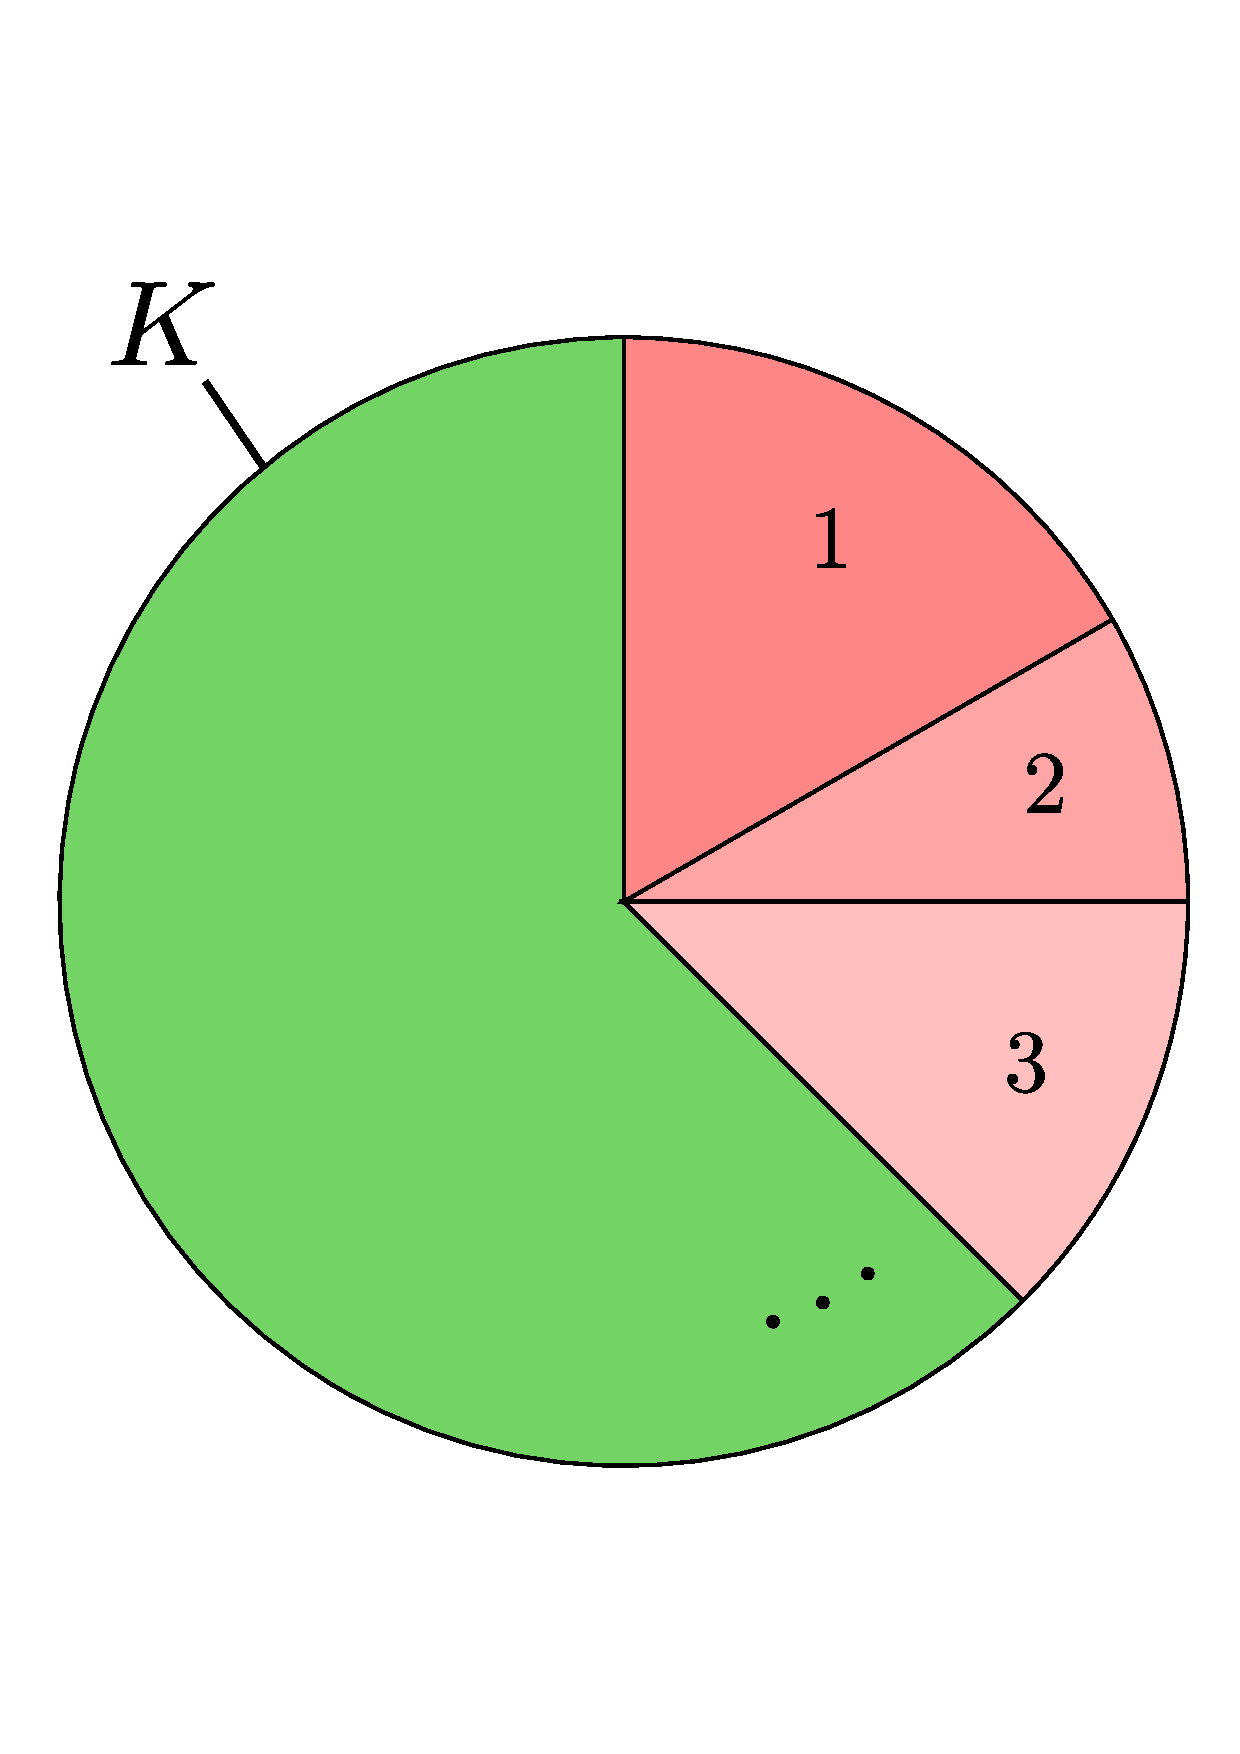
\includegraphics[height=\textheight]{semantics/img/weak_bisimulation.pdf}
	\end{center}
\end{frame}

\begin{frame}
	\frametitle{Bisimulations}
	\uncover<+->{
		\begin{definition}[Weak Bisimulation]
			Let $R$ be a binary relation.
			If $\pair{K, G} \in R$, then
			\begin{enumerate}[i)]
				\itemspacing{7pt}
				\item[] Let $G' = \wh(G)$
				\item $\resN{G'} \sqsubseteq K$
				\item $\pair{K - \resN{G'}, G'} \in R$
			\end{enumerate}
		\end{definition}
	}
	\uncover<+->{
		\begin{theorem}
			Let $R$ be a weak bisimulation.
			Then \[ \pair{K, G} \in R \land G \models B
			\implies \smtx{\while{B}{P}}(G) \sqsubseteq K \]
		\end{theorem}
	}
\end{frame}

\begin{frame}
	\frametitle{Bisimulations}
	\begin{center}
		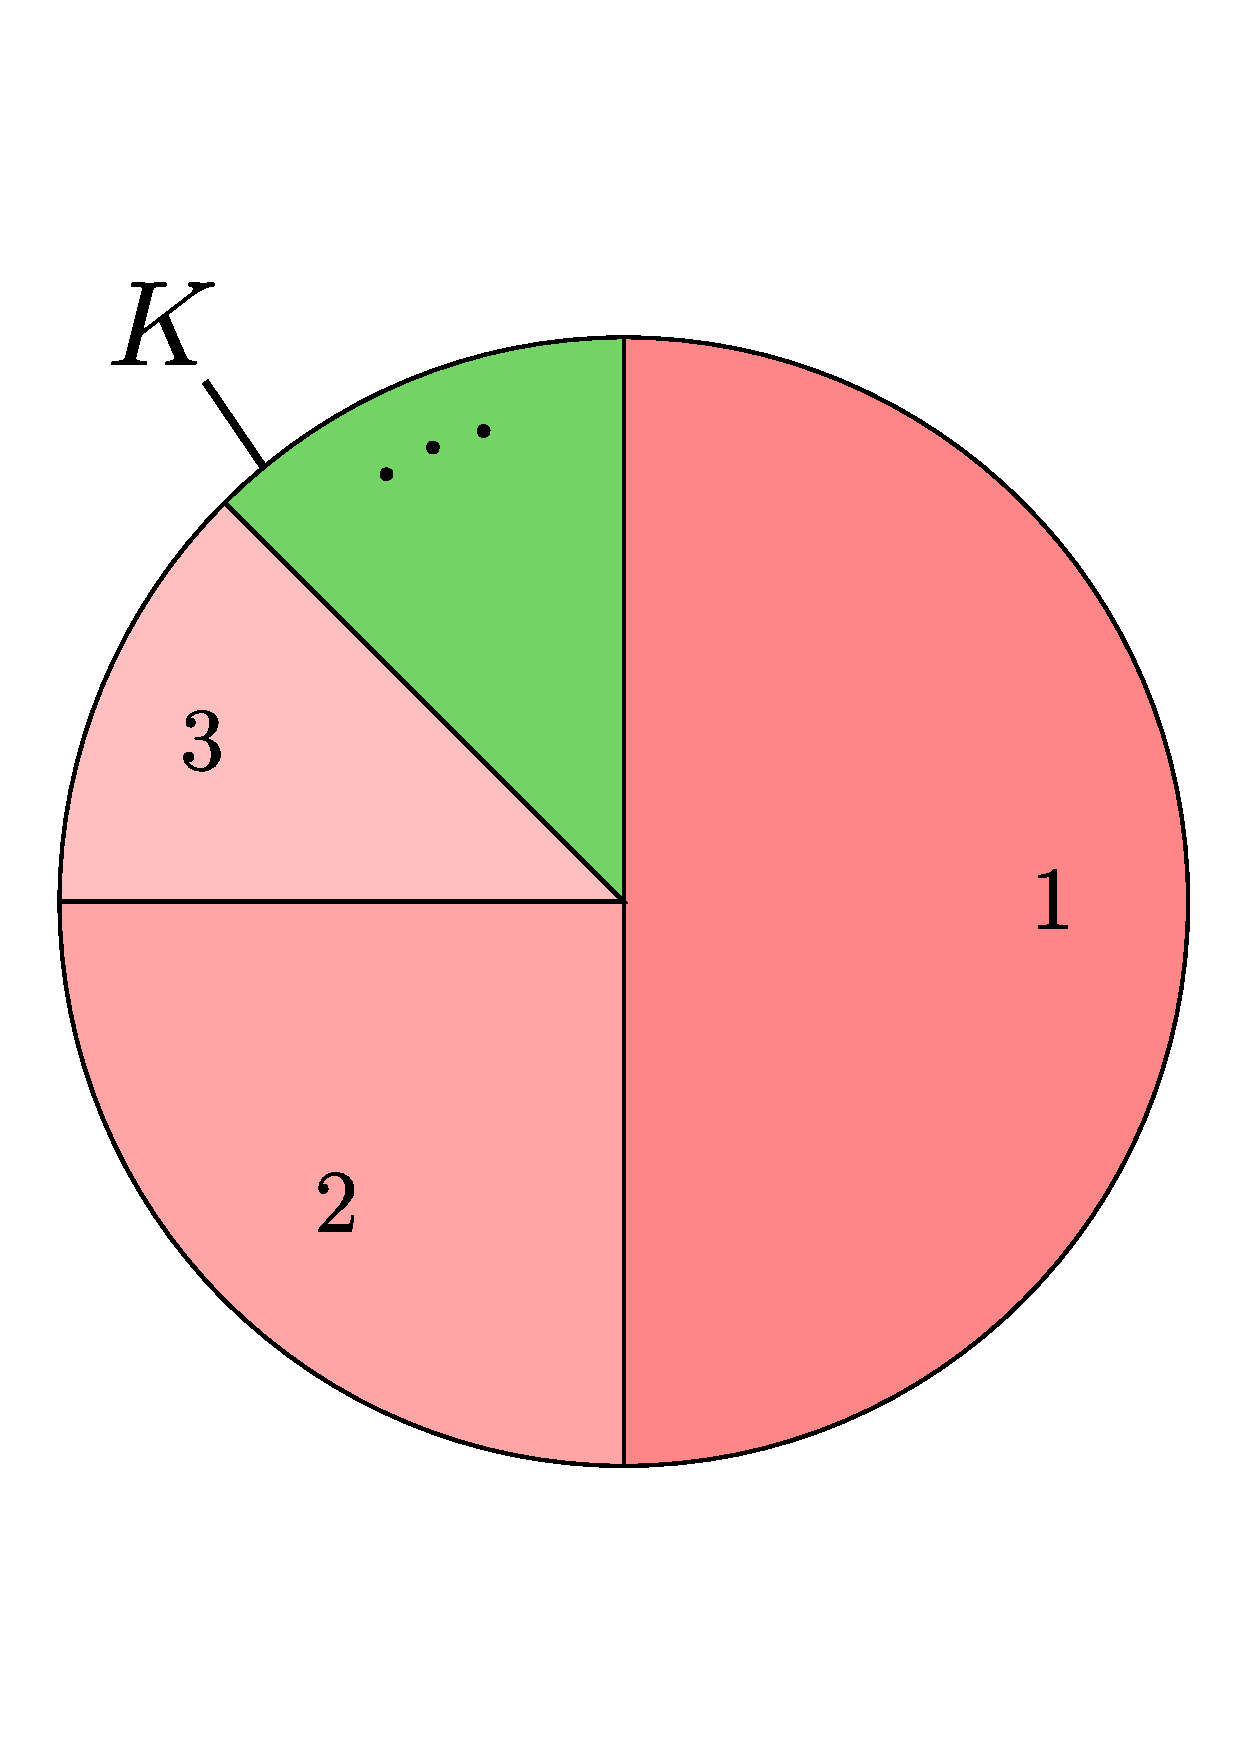
\includegraphics[height=\textheight]{semantics/img/strong_bisimulation.pdf}
	\end{center}
\end{frame}

\begin{frame}
	\frametitle{Bisimulations}
	\uncover<+->{
		\begin{definition}[Strong Bisimulation]
			Let $R$ be a binary relation and $\varepsilon \in (0, 1)$.
			If $\pair{K, G} \in R$, then
			\begin{enumerate}[i)]
				\itemspacing{7pt}
				\item[] Let $G' = \wh(G)$
				\item $\resN{G'} \leqD K$
				\item $\pair{K - \resN{G'}, G'} \in R$
				\item $\left| \resN{G'}\right| \geq \varepsilon \cdot \l| K \r|$
			\end{enumerate}
		\end{definition}
	}
	\uncover<+->{
		\begin{theorem}
			Let $R$ be a strong bisimulation.
			Then \[ \pair{K, G} \in R \land G \models B
				\implies \smtx{\while{B}{P}}(G) = K \]
		\end{theorem}
	}
\end{frame}

\begin{frame}[fragile]
	\frametitle{Bisimulations}
	\begin{lstlisting}
 while (F = 0) {
   {X := X + 1}[0.5]{F := 1}
 }
	\end{lstlisting}
	\begin{itemize}[<+->]
		\itemspacing{10pt}
		\item $ G = 1$, $ K = \frac{1}{2 - X} $
		\item Bisimulation: $ R = \l\{ \pair{K, G}  \r\} \cup
			\only<+->{
				\l\{ \pair{
					\alert<+>{ \res{\frac{1}{2 - X}}{X \geq n} },
					\alert<+>{ \half^n \cdot \l( X^n F^0 + X^{n-1} F^1 \r) } } \ 
					\middle| \ n \in \N_{>0} \r\} 
			} $
		\item $R$ is in fact a strong bisimulation ($\varepsilon = \hf$)!
		\item $ \smtx{\while{F = 0}{\ldots}}(1) \sqsubseteq K $
		\item $ \smtx{\while{F = 0}{\ldots}}(1) = K $
	\end{itemize}
\end{frame}



\section{Contribution}
\begin{frame}
	\frametitle{Contribution}
	\begin{itemize}%[<+->]
		\itemspacing{20pt}
		\item Semantics for negative variable valuations with closed forms
		\item Deeper understanding of two relevant programs
		\item Comparison to an established semantics
		\item Novel approach for finding loop semantics
	\end{itemize}
\end{frame}



\begin{frame}
	\frametitle{\ }
	\begin{center}
		\LARGE Thank you for your attention!
	\end{center}
\end{frame}


\begin{frame}
	% empty frame
\end{frame}


\begin{frame}
	\frametitle{Wp-semantics}
	\begin{enumerate}
		\itemspacing{10pt}
		\item Expectations: $ E = \{ \S \to \R_{\geq 0} \} $
		\item $ \operatorname{wp} \colon E \to E $
		\item $\wp{\nop, f} = f$.
		\item $\wp{\abort, f} = 0$.
		\item $\wp{X := e, f} = f[X/e]$.
		\item $\wp{P; Q, f} = \wp{P, \wp{Q, f}}$.
		\item $\wp{\ifp{B}{P}{Q}, f}
			= [B] \cdot \wp{P, f} + [\lnot B] \cdot \wp{Q, f}$.
		\item $\wp{\{ P \}[p]\{ Q \}, f}
			= p \cdot \wp{P, f} + (1-p) \cdot \wp{Q, f}$.
		\item $\wp{\while{B}{P}, f}
			= \mu X. \l( [B] \cdot \wp{P, X} + [\lnot B] \cdot f \r)$.
	\end{enumerate}
\end{frame}


\bibliographystyle{alpha}
\bibliography{literature}


\end{document}



















